\documentclass{l4proj}
\usepackage{url}
\usepackage{indentfirst}
\usepackage{graphicx}
\usepackage{wrapfig}
\usepackage{caption}
\usepackage{float}
\usepackage{listings}
\usepackage{courier}
\usepackage[svgnames]{xcolor}
\usepackage[colorlinks=true,
			linkcolor=DarkRed,
            urlcolor=Navy,
            citecolor=DarkGreen]{hyperref}

\begin{document}
\title{Level 4 Project Report - A Large Scale Pedometer Application}
\author{David Mcinnes\\ \\0901288m@student.gla.ac.uk}
\date{28th March 2014}
\maketitle

\begin{abstract}

This report describes Hotsteps - an application with a number of aspects - a pedometer application, a website and associated backend software. The user places the app running on their phones and leave it running over the course of the day. It tracks the number of steps they make each day as well as the locations that those steps occur in. This information is then synced with a database located on a central server. A supplementary website uses this information to provide information to the user, such as Leaderboards, personal step counts and Heatmaps showing the areas with the most user activity. The application and website are designed to motivate users into haveing fun and also to create a byproduct, that by-product being the data about steps totals and times, and the location/heatmap data. The app implemented was a good start in developing such a system, but would require additional and more fun features, improved battery life and mitigation some of the privacy concerns uncovered by the application evaluation as it stands.

\end{abstract}

\renewcommand{\abstract}{Acknowledgments}}
\begin(abstract}

I'd like to thank my supervisors, Dr. Alistair Morrison and Dr. Matthew Chalmers and everyone wio helped me when I was stuck, and took part in my evaluation.

David McInnes

\end{abstract}

\educationalconsent
\tableofcontents
%==============================================================================
\chapter{Introduction}
\pagenumbering{arabic}

The aim of this project was to produce and implement a large scale pedometer app using phones and the Internet in order to provide a large scale infrastructure for pedometer usage. This is interesting because fitness and wearable technology is going to be an ever increasing area of importance in technology and Human Computer Interface. The near ubiquity of Gyroscopes and Accelerometers in devices such as modern smartphones and tablets mean that this is more feasible than ever before. Additionally, some high end smart phones as of 2014 have included 'Coprocessors' in order to provide a specialised processor to facilitate the tracking of such user activity. The iPhone 5S has this ability, as well as some Android smartphones. 

The premise of the application was such that users would prefer to not have to carry around separate devices in order to track their walking activity - it would be good if one device that eveyone carries around regardless was used. In today's world, most people carry around mobile phones, with most of these being smart-phones in 2014. This means that the modern mobile phone with its near ubiquty and in-built Accelerometer and Gyroscope is the perfect candidate for this. Instead of a seperate device, just use the mobile that most people have in their pocket.

\section{Background}

A current area of intense research and interest in the field of Human Computer Interaction is wearable technology. Items that purportedly increase the users likelihood of carrying out exercise are increasing in popularity. Many applications, features and products have been introduced in the past couple of years such as endomondo that are designed to gather information about the users physical habits. 

Wearable technology and technology that is designed to increase the users health levels is going to be an increasingly important part of technology as time goes on - it is possible that software such as this could be of a massive benefit to health in general.

With this in mind, there are different ways to provide a niche for a new Pedometer application. It would be interesting if there was a communal way of tracking all of the users of an application communally, with communal information about usage statistics amongst all of the applications users. This could be useful in a whole variety of contexts. If users liked it as a method of promoting regular walking activity, then it could be further expanded to support this usage. Additionally, the location and step tracking throughout the day provides a number of possible benefits to numerous companies or public bodies that might be interested in seeing where users walk throughout the day, and how much walking people are doing. For example, prospective businesses may be interested in viewing what areas are popular with walkers at what time, on order to get an idea of where might be an appropriate 

In the next year or so, the prevalence of such devices will increase massively in everyday usage, meaning that there is likely to be an increase in demand for apps such as Pedometers and fitness trackers. 

The application and website has many uses.

\section{Project Outline}

The goal of this project was to create a pedometer for Android based phones that runs in the background over the user's day, logging useful data about the number of steps the user is making every hour, and also track the coordinate location of those steps. When the user leaves the house in the morning, they turn the application on, and they simply leave it running whilst they go about their daily business. When running in the background, the application tracks the number of steps the user is making and uploads them to a central server hosted by the department every ten minutes. In addition to tracking the number of steps, the application also regularly captures the location of the user as they walk around. These locations are stored until it is time to sync with the server. In conjunction with the application, a website was also implemented that complements the application. Users can use the same login information from the application in order to access their information on the website. This website contains aggregated information amongst all of the users of the application, as well as their own information. Users can view Heatmaps that use the location information uploaded from the app. These heatmaps display the most popular areas that users frequent. The standard Heatmap created are that of aggregated data for all of the users, and your own information per day. Users can also create personalised heatmaps between any new time frames.

The reason that this app was implemented was as a way of getting data about number of steps made per day during 15 minute intervals, and the locations of those steps to be displayed in a Heatmap. The goal of this project is not to propose a specific use for this data, though some ideas will be described, but also to implement a system that promotes the usage of the application in order to harvest this data from users. By adding data tracking features like leaderboards, steps by day and aggregate all-user data it was hoped that the user would enjoy this enough for it to be a worthwhile system to harvest this data, followed up by an evaluation to find out what users liked, disliked, and felt concerned about. 

Battery Life
Is it interesting enough?
Privacy concerns?

\section{Document Outline}

The Literature Review takes a look at previous similar research and applications in the field of activity/location tracking, and how this previous work relates to the themes examined in this project.

The Requirements chapter describes all of the functionality that it was necessary to be integrated into the Android application and website.

The Design chapter goes through the choices of features and technologies used in the project, and why those features and technologies were chosen

The implementation chapter goes through the code internals and gives an overview as how to how the project worked and was implemented.

The Testing chapter

The Evaluations.

INSERT INFO ABOUT THE REST OF THE DOCUMENT!

%==============================================================================

\chapter{Literature Review}

Before undertaking the project it was necessary to undertake a review of recent literature from similar topics and products.

There were a variety of research papers that informed my approach to designing and implementing the system and designing/carrying out the evaluation upon the system. In this section, each of these papers will be discussed and how their findings relate to the system.

\section{Games with by-products}

\subsection{The "ESP" game}

Given the focus on getting users to use the application in order to produce a by-product (the step and location data), a seminal 2004 paper on an interactive system (in this case a game called "ESP") that simultaneously is enjoyed by the user and gives a valuable by-product is 'Labeling images with a computer game' by Ahn and Dabbish [1]. The paper describes a game whereby the user is presented with photos and enters 'keywords' for that image, whilst getting a simultaneous user to "agree" on a keyword. Say for example the users are presented with a picture of a brown purse. Words that might come to mind are "purse", "bag" and "brown", which is entered by the first user. The first guess typed in by the second user is "handbag", which doesn't match any of the input keywords by the other user. The second user then inputs "purse", which does create a keyword match between the two users. In reward for matching each other, both of the users are rewarded with a certain number of points. If they can agree on fifteen images, then both users get a large number of bonus points. Users are promoted to continue using the application by the presence of a "thermometer" on screen that continually fills the closer the users get the completion. The game is made more complex by the presence of up to six "Taboo words" - words which have already been agreed upon many times for that image and hence are not allowed to be used again. This increases the richness and number of the labels for each image in the game.

The hugely beneficial by-product from the ESP game is that of labelling and categorising images on the internet, ideally those images indexed by search engines. Doing so would improve image search reults massively. Traditional techniques such as computer vision and analysis of the text nearby images had not been successful, but using the human mind was considered perfect for this task. When the two users agreed on a image description, this was typicaly a good label for that image. A major aspect of the evaluation of the ESP game is that the users are never asked to enter keywords describing the image on screen, but that evaluation of and usage of the game has shown that users do in fact enter accurate labels for the images in the game. Data showed that the game could be agreed upon as being fun - users sent a lot of time playing - 50 hours in some cases! - and most people played at least once. 1.3 million labels were created with only 14,000 users, with the assumption from that being users enjoyed the game. The game was very successful at acheiving high quality by products, the descriptions of images were accurate and helped image labelling, and at the rate of use at the time of the evaluation, could have indexed all of the images on Google images within weeks. As the authors concluded, what would normally be considered tedious work had been transformed into "something fun to do".

\subsection{Eye-Spy}

Another paper that builds on the "ESP" game describing a game with a by-product is "Eyespy: Supporting Navigation through Play", a 2009 paper by Bell et al [2]. The paper describes "Eye-spy", a game designed to extract picture and location data from users. Whilst using the app, players 'tag' geographic locations with pictures or text, and when other users visit that tag, they can "confirm" them, gaining points for doing so, and also verifying the accuracy of the tagging. Eye-Spy was judged to be successful, not only as a game (users commented that using the app gave them great enjoyment in visiting areas they had visted many times before, allowing them to view locations in a new light), but also in creating useful augmentations of maps with the accuracy of crowd confirmed correctness of images.

\subsection{Crowdsourcing}

Both of the above papers use the concept of 'crowdsourcing' in order to create and extract data about images or the environment. Crowdsourcing is a technique with growing popularity.

\subsection{}

\section{Motivating Use}

Obviously in order for users to get the data they must be at least semi motovated to putting their time and effort to use the app. A growing category using technology in recent years is that of the 'Quantified Self', where technology is incorporated into tracking of user activities in order to provide a benefit to the user. This could include logging of the users diet for weight loss and diet purposes, as well as activity tracking, whether that be running or walking. Example of such devices on the market include the FitBit and Nike Fuelband.

\section{Previous Systems - Research}

\subsection{Ubifit Garden}

UbiFit garden was an early smartphone application that aimed to provide a stimulus to increase user activity of the mobile phones. Given the era that this application was develeoped in, the application requires additional hardware bolted onto the back of the phone. Given modern conveniences, many people would consider this to be an unacceptable drawback to the application, but for a time when smartphones did not have included accelerometers and gyroscopes to be able to internally handle such applications.

Ubifit Garden was designed to be used by the user throughout their day to day business 

\subsection{Shakra}

Shakra was a research paper published in 200

\subsection{Houston}

This was a research paper published in 2006 

\section{Previous Systems - Commercial}

\subsection{Nintendo 3DS Pedometer}

There are a number of products on the market that act as a pedometer for users to keep track of their steps. An example of this is the 'Activity Log' application in Nintendo's 3DS Handheld video game system. Whilst the system is on standby in the users pocket whilst they walk around, it tracks the number of steps they are making throughout the day. Ostensibly designed to promote user activity through walking, the application contains a number of elements of note. Users are motivated into using the application by being given more play coins the more steps they make each day, up to a total of ten. These play coins can be used to buy items to make progress in games, or receive unlockable content. This provides additional enjoyment to the user, and by carrying out that task, the user receives a benefit to them. The activity log also contains a by-product with a benefit on Nintendo's part, as by the act of having the user walk around with the system in their pocket, Nintendo gains valuable data through the 'Street Pass' application in addition to motivating users to carry around their video game system all of the time, and at the same time providing benefits to users.

\subsection{Endomondo}

\section{Privacy}



%==============================================================================

\chapter{Requirements}

\section{Non-functional Requirements}

\subsection{Work on a large scale}

\subsection{Security}

\section{Functional Requirements}

\subsection{Android Application}

In order to be able to track the users steps, it was necessary to implement a Smartphone application that would be running whilst the user had theur smartphone in their pocket. The app must work in the background whilst running in the users pocket. It should be relatively conservative on users battery life, and also must be able to track the users current location whilst using the app on a regular basis. There must be a log in screen that allows users to enter their username and password to enter the app and associate their usage of the app with their own account. Additionally, there must be the functionality for users who do not have an account on the service to be able to create one. Once the user has been logged in, the application should start tracking the number of steps they are making and be able to display this to the user in a visually obvious manner. Additionally, it should provide the ability to manually sync with the server and provide a visual indication of daily leaderboards and how many steps the user has made on previous days, though it is intended that the majority of the data viewing capabilities will be reserved for the website due to a limitation in development time.

\subsection{PHP Backend}

It was necessary to implement a backend server to provide the data services for the Smartphone application. This will receive the data sent over the network from the application and handle it in the appropriate manner. When an HTTP request is sent via the app to update the server about a users step total or location data, then these scripts handle the data sent using the requested script. This could be adding data to the database, querying the database to display information on the website or application, or carrying out authentication and cookies for the website.

\subsection{Database}

It was necessary to design and implement a database to store the data required for the application and website. This database should store user accounts, assign them a userID, and store all of the steps by day and a list of locations indexed via date and time in order to provide information for the heatmap data. The data would be added and queried to using the PHP back-end and this will provide and receive data to the app and website.

\subsection{Website}

In order for the user to have a way to access the information, it would be necessary to design and implement a website that will allow users to view their step totals for days, and also to display Heatmaps that make use of the location data that is harvested by the app.

%==============================================================================

\chapter{Design}

\section{Technology Choices}

\subsection{Choice of Mobile Operating System}

Before development began, it was necessary to decide what technology and OS the app would be implemented in. Given the popularity of iOS and Android in modern mobile phones, I decided to choose between these two. Development in iOS uses the Objective C language, which is predominantly used by Apple. I didn’t have any experience developing using the Objective C. Additionally, iOS development requires the use of the XCode IDE, which is only available on Mac OS X.  While this would be possible in my circumstance, it would be more logistically challenging given that it was likely that development would take place on a number of different machines. However, with iOS there are a far smaller number of possible devices that I would have to design around and test for.

Android development is cross-platform on Linux, OS X and WIndows, meaning I could use any computer for development. This would make development logistically easier. Additionally, Android development uses the Java programming language, which I have a lot of experience in, having done it in many courses and having used it as the implementation language for my Level 3 Project. There are a lot of tutorials and guides available for both iOS and Android development.

Given the available choices, I decided to develop the system for Android OS due to my experience with Java, making it less likely that development would reach a snag or be slower due to my inexperience with Objective C. In future, the app could be ported to iOS if usage of he app was shown to be popular.

When considering the overall design of my application, it was necessary to consider many different factors. A major one of these was the prevalence of many differing factors.

Before development began, it was necessary to decide what technology and OS the app would be implemented in. Given the popularity of iOS and Android in modern mobile phones, I decided to choose between these two. Development in iOS uses the Objective-C language, which is predominantly used by Apple. I didn’t have any experience developing using the Objective-C. Additionally, iOS development requires the use of the XCode IDE, which is only available on Mac OS X.  While this would be possible in my circumstance, it would be more logistically challenging given that it was likely that development would take place on a number of different machines. However, with iOS there are a far smaller number of possible devices that I would have to design around and test for.

Android development is cross-platform on Linux, OS X and WIndows, meaning I could use any computer for development. This would make development logistically easier. Additionally, Android development uses the Java programming language, which I have a lot of experience in, having done it in many courses and having used it as the implementation language for my Level 3 Project. There are a lot of tutorials and guides available for both iOS and Android development. One of the major obstacles involed with choosing Android development over iOS is that there are a much greater number of devices that use Android at any given time versus devices that use iOS. Whilst iOS devices are generally all within the high end range of current technology, Android devices can vary wildly in CPU speed, internal memory, and screen resolution. This means making a possibly complex decision about which type of devices to target development for.

Given the available choices, I decided to develop the system for the Android Operating System due to my experience with Java, making it less likely that development would reach a snag or be slower due to my inexperience with Objective C. In future, the app could be ported to iOS if usage of the app was shown to be popular and more data could be logged through such a development.

\subsection{Choice of Database and Server technologies}

Given the large scale nature of the application, it was necessary to have a centralised server that handles all of the POST requests made by all of the users of the application. This behaviour would be achieved via a number of PHP scripts designed to handle the situations that will arise from usage of the application. This same server would host the database and the website, allowing inter-operability between the website and the application through the centralised database.

\subsection{Database Design}

When beginning to consider storing the user data, it was necessary to design a Database that would effectively hold all of the necessary data, be able to query that data in a reasonable timeframe given the mobile nature of the project.

\begin{figure}[H]
\centering
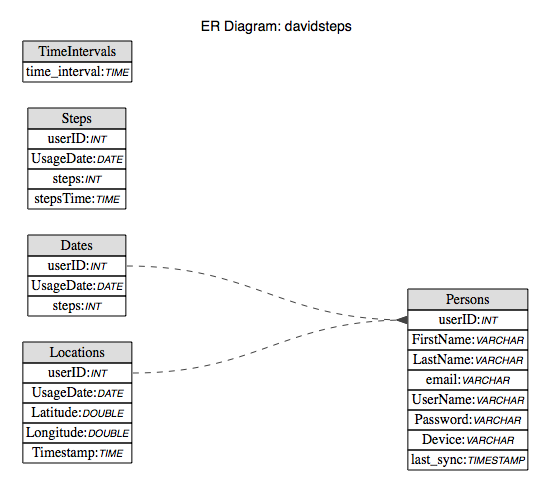
\includegraphics[scale=0.5]{images/screenshots/erdiagram.png}
\caption{\textbf{Displays the Entity Relation diagram for the Database designed}}
\label{design:erdiagram}
\end{figure}

A diagrammatical representation of the design of the Database is seen in Figure \ref{design:erdiagram} in the form of an ER (Entity-Relationship) diagram.

\subsubsection{Users Table}

\begin{figure}[H]
\centering
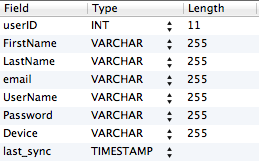
\includegraphics[scale=1.0]{images/screenshots/usersscreen.png}
\caption{\textbf{Displays the attributes of the Users table of the Database, as well as their type.}}
\label{design:usersscreen}
\end{figure}

The table Users stores all of the data about the usernames of the app. userID, Firstname, Surname, Email, Username, Password (stored as an SHA-256 Hash), and a Timestamp signifying the last time the user pinged to the service, so it can be seen if people are using the application. The attributes and types of this table can be seen in Figure \ref{design:usersscreen}

//INSERT INFO ABOUT Users TABLE HERE!!!

\subsubsection{Locations Table}

\begin{figure}[H]
\centering
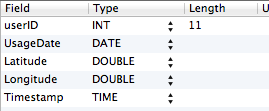
\includegraphics[scale=1.0]{images/screenshots/locationsscreen.png}
\caption{\textbf{Displays the attributes of the Locations table of the Database, as well as their type.}}
\label{design:locationsscreen}
\end{figure}

The next Table is Locations, which stores all of the Latitude and Longitude pairs uploaded to the service. The attributes and types of this table can be seen in Figure \ref{design:locationsscreen}

//INSERT INFO ABOUT Locations TABLE HERE!!!

Each location is associated with a userID, to make it known what user was in this location. This is integral for the website aspect of the Project. Each Latitude and Longitude originates from a user of the application whilst using the application. These are stored as doubles due to the floating point nature of precise coordinates.

\subsubsection{Steps Table}

\begin{figure}[H]
\centering
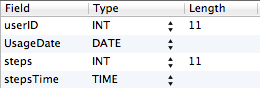
\includegraphics[scale=1.0]{images/screenshots/stepsscreen.png}
\caption{\textbf{Displays the attributes of the Steps table of the Database, as well as their type.}}
\label{design:stepsscreen}
\end{figure}

The final table in the Database is the Steps table, which stores the amount of steps each user has made in a 15 minute interval. Whenever the user uses the service for the first time each day, a record is added in the Dates table for each 15 minute interval in that day. A limitation of this is that a number of records each day will essentially be empty and have 0 steps, taking up storage space for the database. The trade-off was to either make the data harder to traverse and re-assemble when it comes to using that information in the application or website, or save space and make re-assembling the data somewhat harder. Having gone over the different options, the former option was chosen, though there is no technical reason why this cannot be changed in the future if space was becoming an issue. Whenever the app refreshes its sync with the server it checks what 15 minute interval the set of steps occurred in, and add the number of steps that occurred in that set of steps to the total for that 15 minute interval. The attributes and types of this table can be seen in Figure \ref{design:stepsscreen}

//INSERT INFO ABOUT Dates TABLE HERE!!!

\section{Application Design}

For the design of the Android app, consideration was made as to what UI elements should be front and centre of the users view at any given opportunity and started to make some prototypes based upon that. A wireframe showing the initial application design at the Design stage is shown in Figure \ref{design:appwireframe}.

\begin{figure}[H]
\centering
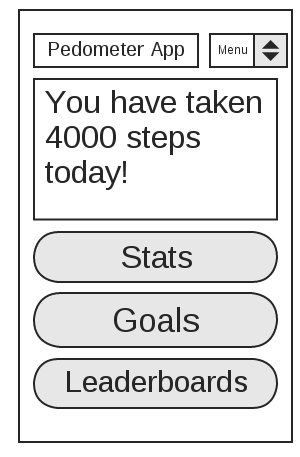
\includegraphics[scale=0.7]{images/diagrams/appwireframe.png}
\caption{\textbf{Wireframe of the User Interface of the Android application during the design stage. The step totals can be seen, as well as the menu dropdown, and options for statistics, goals and leaderboards. Goals was left unimplemented in the final application.}}
\label{design:appwireframe}
\end{figure}

\subsubsection{Step Count}

The main UI element had to be the number of steps for that day. To hit the user instantly with the information as soon as their eyes catch onto the app, the text including the step count was put in the middle of the app in a large text.

\subsubsection{Goals}

Below this, obvious to the user, includes buttons to navigate to the other sections of the application, such as the statistics and leaderboards views. There had been plans to include a button to proposed Goals functionality, that would include a number of goals for the user to complete. The main 

\subsubsection{Statistics}

This screen of the app shows all of the previous days step totals from that user. The goal of this feature is to promote the user into making more steps to match up to their previous days.

\subsubsection{Leaderboards}

The leaderboards screen shows all of the users of the app's step totals for the given day, in descending order. Again, this is a feature designed to promote continued use of the application by users 

\section{Website Design}

The website is designed and all of that garbage.

There were a variety of different factors to be considered for the website aspect of the project. It was an absolute necessity from the beginning of the development process that the account system would be common - users must be able to Log In to both the website and the Android application using the same account.

It was also wanted for the website to be modern and eye-catching. Use up to date web technologies. Bootstrap + JQuery.

\subsection{Choice of Web Development libraries}

I used Bootstrap, JQuery to provide look and feel and functionality for the website. Bootstrap is a front-end framework that provides all of the CSS and Javascript to provide a good looking, responsive website that that has a consistent look and feel, over standard HTML and Javascript components that are liable to look ugly. Bootstrap is a very popular framework, providing a front-end for many commercial websites.

JQuery is a library that extends and adds many features to the Javascript language, adding functionality such as sending POST requests and the like. In the website it is used to send POST requests to PHP scripts that return JSON appropriate to what is currently being viewed.

\subsection{Heatmaps}

Given that there would be heatmaps embedded in the website, it was necessary to think of designs for heatmaps and what might be considered necessary in the design of these. Commonly, heatmaps use a colour scale from green to represent light data coverage, to amber for moderate data coverage, and finally red to represent areas of the highest data concentration. These colours may be standard and appropriate for most users, but some people are likely to have colour blindness and therefore make it difficult to distinguish between or understand the colours represented. Therefore, when choosing a library or toolkit to provide these heatmaps in the finished website, it would be necessary for it to provide an option for colour blindness, as well as the possibility of increasing the radius of each data point on the map, to help people who may not be able to pick out or see the data points as effectively as intended. 

Addtitionally, if there is a lot of data in the heatmap, then there is the functionality to increase the radius of the data points on the heatmap, thereby making them appear much bigger. This has the benefit of making the data look much more obvious if there is little data for that day. 

%==============================================================================

\chapter{Implementation}

In order to successfully implement all of the software required for the project, there were a number of new programming languages and concepts to become comfortable in using. For example, I had no knowledge of PHP but had to learn in order to implement the back end for my project. I followed some tutorials to quickly learn PHP in order to have enough skill to be able to implement what I need to. I carried out development using the Eclipse IDE, the de-facto standard for Android development currently, though alternate IDEs are in development with the mind of replacing this. 

A diagram of the system overview as implemented can be seen in Figure \ref{impl:dia1}. As can be seen, the system consists of two different types of client. Firstly, the app user, who interacts with the server to download their current step information when logging into the app, as well as some basic statistics for view in the application. The second client type, that of the website, interacts with the server back end to query information such as step totals, leaderboard information and coordinates to display on the website heatmaps.

\begin{figure}[H]
\centering
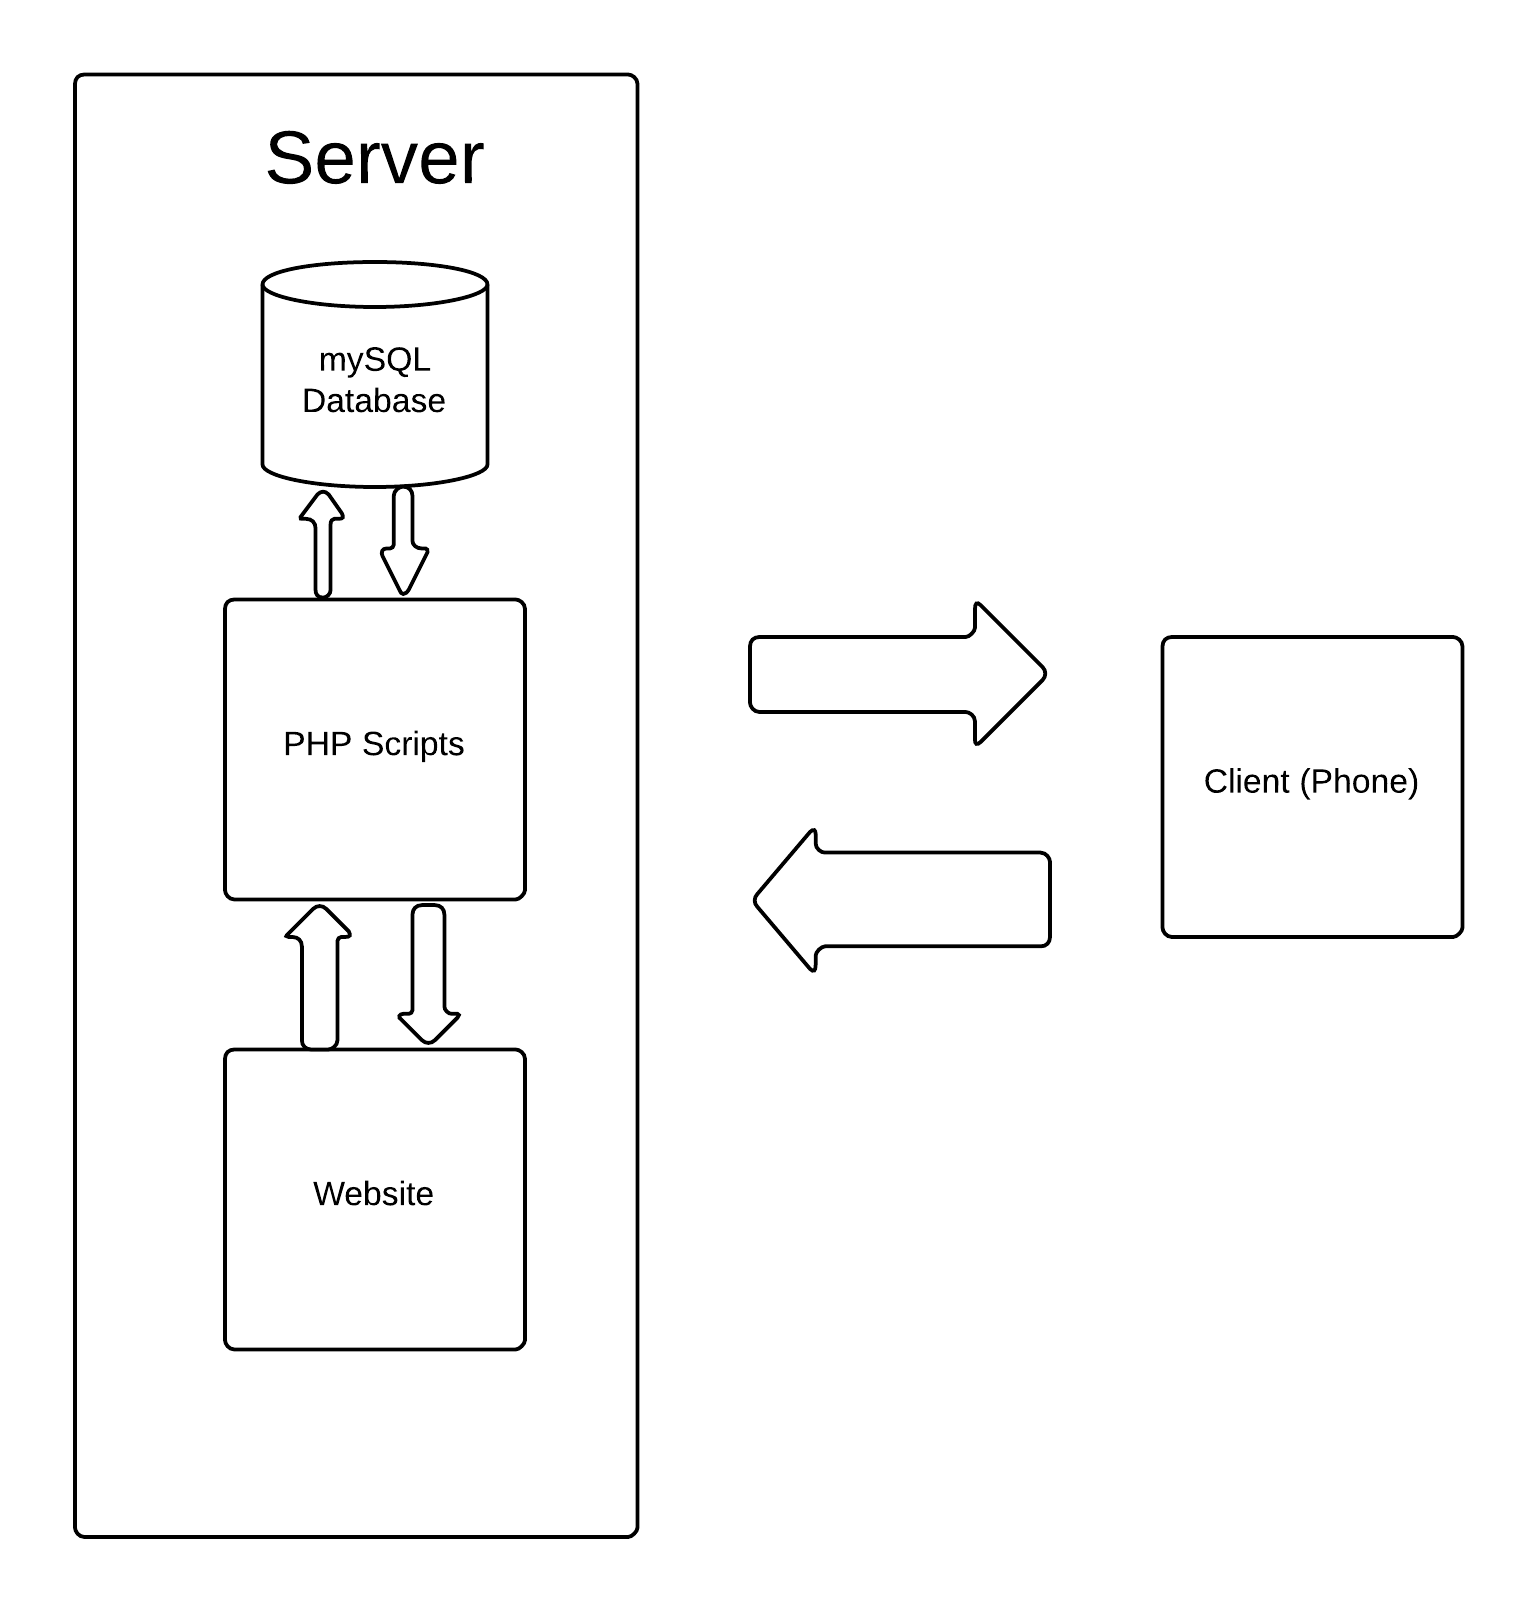
\includegraphics[scale=0.2]{images/diagrams/systemoverview.png}
\caption{\textbf{Diagram of the System Overview. The server which hosts the Website, PHP scripts and Database communicates back and forth with the phone and website acting as the Client.}}
\label{impl:dia1}
\end{figure}

\section{Android Application}

In this section, the implementation of the Android application aspect of the project is described.

\subsection{Implementation Overview}

One of the major concerns throughout implementation of this project was to get the application to such a state whereby battery life is not excessively drained by  near constant usage of the application as it is designed in anticipation of. Modern smartphones generally have relatively poor battery life given their high processing power, high-resolution screens and regular network operations. These network operations can happen regularly, and if not managed in an efficient manner  they can cause a real negative impact towards the battery life of a device. If an application is causing the user's battery life to be at an unacceptable level reguarly, most users would simply rather delete the application than continue using it. Therefore, when making design decisions regarding the User Interace and network operations the main priority in determining the implemented behaviour was that of saving battery life.

The first stage of implementation involved getting to grips with Android development, which I had little experience in. This involved reading tutorials on the Android developers site, which has a good introduction to Android development that teaches me the basics, such as learning about Views and Activities, as well as show to travel between and move data between views using Intents. \textbf{\textit{Views}} are written in Extensible Markup Language (XML) and describe the look and feel of the User Interface. User Interface elements such as TextBoxes and Buttons and GridViews are introduced to the UI here. The behaviour behind the UI elements are implemented in \textbf{\textit{Activity}} files, which are implemented as Java classes. Each Activity class consists of a number of methods that are automatically called.

The application consists of 7 Activity classes. In Android development, files describing the layout, look and feel of the User Interface are written using Extensible Markup Language (XML), which represents different views and UI components in a hierarchical structure. The functionality of the app itself is implemented using the Java programming language. Such a technique seperates the look and feel of the app from the actual functionality - following the principal of separation of concerns. Errors in the UI code doesn't cause errors within the Java code.

Due to the time and location based nature of the application, whenever the location as detected from Play Services changes another object is data is added to the Array consisting of the number of steps in that interval, the time, and the location in question,  and it is obvious as to what type of code is causing the issue when the application has errors and does not compile. 

\subsection{Network operations and \texttt{AsyncTasks}}

Android does not allow Network based operations to occur on the main UI thread. This is the Thread that runs as part of the activity lifecycle. In order to carry out Network operations, Android provides a wrapper for one time use threads that perform a task not related to the UI thread. ASyncTask takes in zero or more objects and uses them to complete a method and another method upon completion of that method. When it is time for the Application to sync with the server, the Array of packets is passed to the AsyncTask, which sends this JSON data to the server via a POST request, along with the userID. The PHP script which is invoked, \texttt{updatedb.php} loops through all of the data objects, and updates the total number of steps for the 15 minute interval signified by the time in the 'steps' table, and adds the location along with the time and the date that it occurred to the locations table. Theoretically, data can be lost using this system. If the request never makes it to its destination or it is corrupt there is no error fixing, no resending, and the data once sent is not recoverable. This was considered an acceptable risk, as none of the data is critical and the odd loss on occasion is acceptable.

\subsection{\texttt{AccountLogin.java}}

When the app is initially loaded without a saved login, the first screen that loads is a Login.java. The User Interface for this view can be seen in Figure X.X. This consists of a standard user login screen, with TextFields for Username and Password. The field for password is a special UI element that covers up the characters entered. If the user does not have an account, they can move to the screen that enables them to create their own account using the 'Create Account' button. Once the user has entered their login details, the system checks using a POST request and response that sends the information to check whether or not the account exists in the database and whether the password corresponds to the one on record. If the login details are not correct, the user is informed through the use of a 'Toast' UI element, which displays a small message that overlays the rest of the screen. Once correct user credentials are confirmed, an Intent is sent to send the user to the main Pedometer screen of the application.

\subsection{\texttt{AccountCreation.java}}

If in the previous screen has sent app execution to the 'Create Account' page, Before this appears, there is an information page that appears about the Terms of Use of the application, which informs users that their location and number of steps will be tracked. If the user disagrees, a Toast appears that informs the user that as they have not agreed to the terms of service, they cannot create an account, and then execution is transferred back to the Login screen. If the user accepts, then they are passed onto the Account Creation form, a screenshot of which can be seen in Figure X.X. This screen consists of a form that prompts the user for the details required by the applicaion and Database for user accounts. 

\subsection{\texttt{PedometerActivity.java}}

The main backbone of the application is that of \texttt{PedometerActivity.java}, which provides the code for the main view of the application. This is displayed after the user logs in. Once the screen appears, an object of type \texttt{StepCounter} is created that begins to track the users step count. This class displays the interface defined in \texttt{pedometeractivity.xml}, as seen in Figure \ref{impl:dia2}. There are a number of buttons the user can click on this screen. 'STATISTICS' will take them to a page that allows them to view all of their statistics, and 'LEADERBOARDS' takes the user to a page that lets them see that day's leaderboards. 

\begin{figure}[H]
\centering
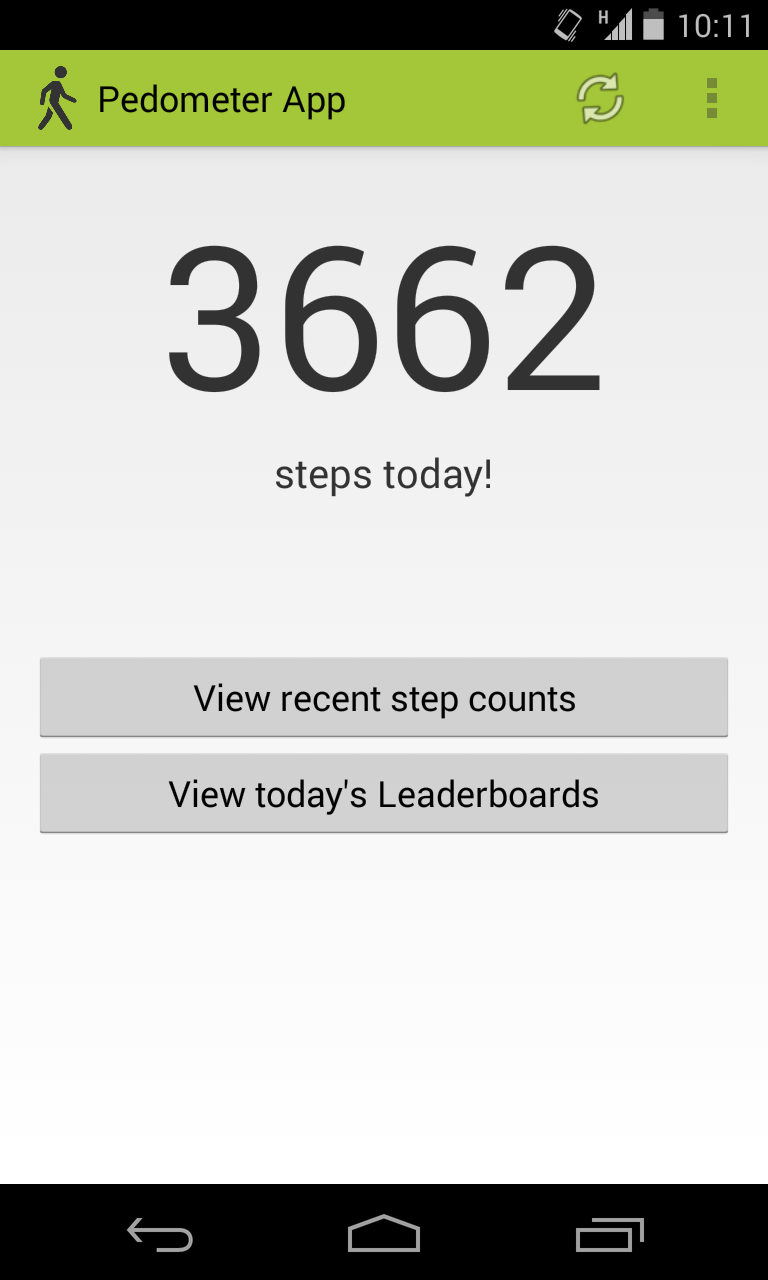
\includegraphics[scale=0.3]{images/screenshots/appscreen.png}
\caption{\textbf{Screenshot of the main view of the Android application, defined in pedometeractivity.xml and PedometerActivity.java}}
\label{impl:dia2}
\end{figure}

Whilst the app is running, whenever the location services integration detects a change in location, a callback method is called that stores the current time, the amount of steps since the last change in location, and the current Latitude and Longitude. This information is then encoded as a \texttt{JsonObject} and this object is stored in a \texttt{JsonArray}. 

In the background, the application is tracking the number of steps. There are a number of different aspects to the updating of the server with this information. There are 2 threads on a timer that are running alongside the app. The first of these updates the User Interface with the day's step total as you are walking around. The second of these sends all of the data packets (Stored os JSON) in the data array up to the server to be added to the Database. 

\subsection{\texttt{SessionManager.java}}

It was necessary to provide a local data store on the device itself in order to save data that the user will not want to enter everytime, such as their login details. These are stored using Android's \texttt{SharedPreferences}, which saves data as Key-Value pairs locally on the device. In this scenario, if the user logs in and closes the app without intentely logging out, then their user data is saved and upon reopening the application, their profile logs in automatically. \texttt{SharedPreferences} also provides benefits for the internal transfer of data within the application. Instead of having to transfer pertinent information between views through the use of Android Intent calls, it could simply request the appropriate information through a call to the \texttt{SharedPreferences}. The main use for this in the application is to get the userID which is received from the database when the user logs in and is stored as a \texttt{SharedPreferences} Key-Value. Whenever one of the views in the app needs the userID of the current user, it makes a request to \texttt{SharedPreferences}, and receives the userID. In addition to being easier to implement and manage than Intent passing, this also reduced the possibility of user data becoming corrupted, as instead of being passed between views contantly, the values are set upon loading and simply called upon when needed.

\subsection{\texttt{StatisticsActivity.java}}

This class displays an interface consisting of a ListView defineed in statistics.xml. A ListView is a standard Android UI element that can be populated with content and which takes the form of a list that can be scrolled over by the user if it does not fully fit the screen of the device. When this class is loaded it sends a POST request to \texttt{jsonscript.php} containing the current userID as received from the central \texttt{SharedPreferences} store that returns all of the previous days Step Counts for that user as a list in JSON format. The JSON list is then parsed and added as elements to the \texttt{ListView} which are then displayed in the list.

\subsection{\texttt{LeaderboardActivity.java}}

\texttt{LeaderboardActivity} displays a \texttt{} as defined in \texttt{statistics.xml} to display the list of users who have used the app on the day in question and displays their step counts in descending order as a Leaderboard. This class sends a POST request to leaderboards.php hosted on Tethys which returns as JSON a list of users in descending order of Step Count for that day. The JSON is then parsed and the content extracted is reformed as readable text and added to the ListView and displayed. A screenshot of this screen can be seen in Figure 

\begin{figure}[H]
\centering
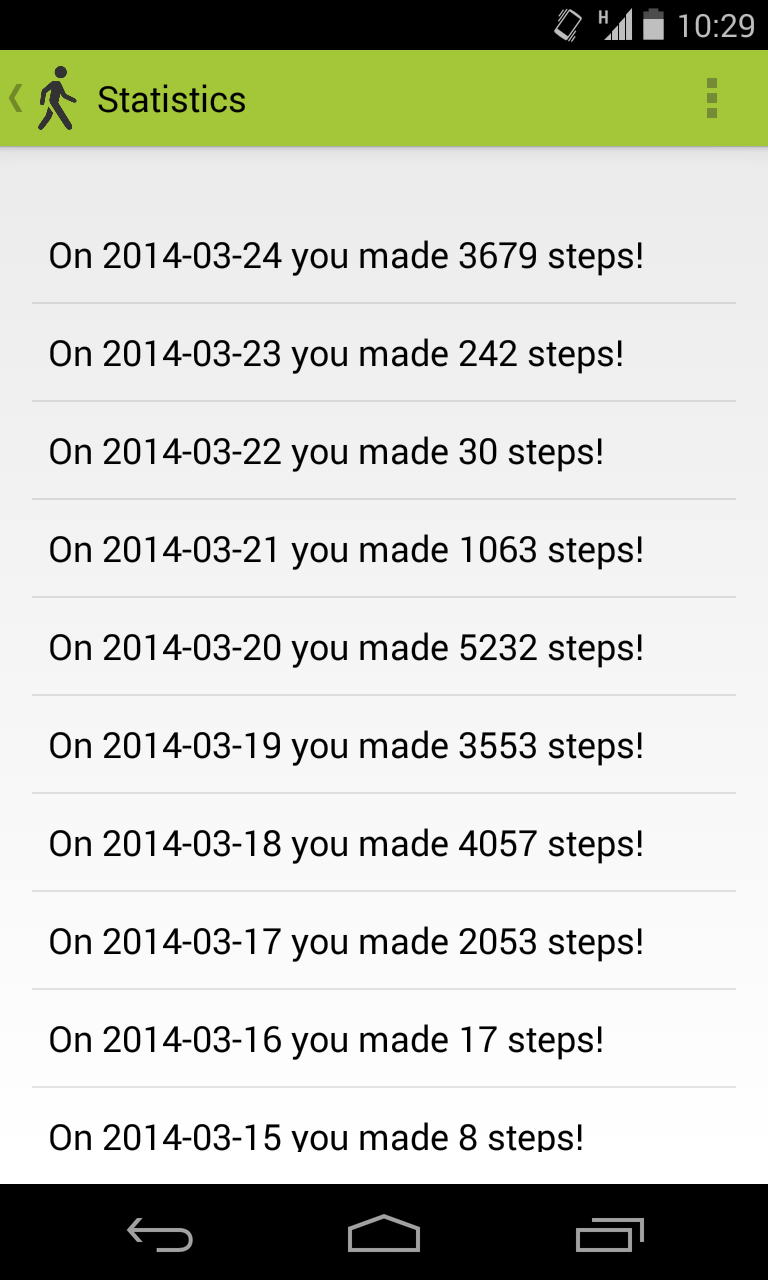
\includegraphics[scale=0.3]{images/screenshots/statisticsscreen.png}
\caption{\textbf{Screenshot of the Screenshot view of the Hotsteps Android application, defined in statistics.xml and StatisticsActivity.java, showing the previous day's step totals for that user of the app.}}
\label{impl:dia23}
\end{figure}

\subsection{\texttt{Agreement.java}}
 
Displays a view showing the user the Terms of Use and buttons to agree or disagree. Handles the acception of rejection of the user agreement when creating an account. IF the user agrees to the Terms of Use as displayed. then an Intent moves execution to AccountCreation. If the user disagrees, then similarly an Intent rakes execution back to the login page and displays a Toast that indiciates that since they disagreed, they cannot use the app.

\subsection{\texttt{StepCounter.java}}

The pedometer code that I was offered was written by Mattias Rost, and had been in use by the department for several other projects before my own. This code was not very well documented, however, and I was unsure how to instantiate the code, make it run and begin to track the users steps.  After some correspondance with the original author of the code, it became apparent how I should edit the code in order to make it suit my circumstances. The code I had been given included code to facade with a Database already present on the local device, but in my Application, this was not needed as it would be hooking into a Database that was already present.

Another problem I encountered was how to actually instantiate the Pedometer code so that it was tracking steps as the user walked. It turned out that it used a slightly unusual method of instantiation that involved toggling a Boolean when it was turned on.

\subsection{Android Version 3.0 Limitation}

The application developed only works on Android devices with Android version 3.0 and above. This limitation was chosen based upon updated UI guidelines and technology introduced with that update, which introduced the Action Bar. In addition to having two support two different UI styles if a version for devices older than Android 3.0 was developed, this would also add additional development time and effort in order to support a limited number of older phones with less effective technology and battery life, which would not provide the best performance for the application. This decision minimised excessive development time and ensured the ability to adopt the more modern APIs available.

\subsection{Google Play Services}

Google Play Services is an API available for usage by developers that enables applications to be able to access many Google provided services. In my application, Google Play Services is used to provide and access the location data whilst the user is using the app. Google Play Services is only available on official Android phones, and not those that only support the Android Open-Source Project (AOSP). This is a minor limitation to the number of devices that could be used in this application.

\section{Back end and Database}

\subsection{Database}

The database necessary to support the functionality of the application and website by storing user information. The database used for this project is a mySQL Database hosted on a DCS server named Tethys, which also stores the PHP scripts and website.

The database was implemented on using a mySQL client named Sequel Pro. mySQL was chosen as the DBMS due to its availabilty on the server used and also due to it being open-source and not having any licence fees or the like associated with its use. At first, before the database had been made available on a centralised server, the database was stored on a local machine, but when Tethys became available, the Database was exported onto it, meaning that the app could be used from anywhere with an active internet connection.

Each table was created using the CREATE TABLE command in mySQL. The Persons table has the attribute userID as its primary key, and all of the other tables use this as a Foreign key. An ER diagram showing the Database design can be seen in Figure \ref{design:erdiagram}.

\subsection{Back-end}

The back end is written using the scripting language PHP. PHP is a recursive backronym for "PHP: Hypertext Preprocessor". Scripts hosted on the server provide access to information from the website and the application. There are a group of scripts assocated with serving the application, and a group of scripts that are associated with providing content for the website. 

//LIST OF ALL THE SCRIPTS GO HERE!!!!!1111

The scripts on the server are hit by using HTTP Post requests from the Android app and the website. This HTTP is sent using Apache's HTTP library provided with the Android SDK in the Application. Along with the request are POST parameters that include the information that is required to query the appropriate data in the script. For all of the scripts, these return encoded JSON to display the appropriate information in the application or website, and also to confirm whether the correct results were achieved.

The scripts used for the Website are also hit using HTTP Post requests. This HTTP is sent to the server in the form of JQuery POST requests. JQuery is an API for the Javascript programming language that adds features to the language and greatly improves the interactivity between websites and users, and database between website.

The majority of the PHP scripts use the more modern and secure 'mysqli' or mySQL Improved library to query the Database. The other library has been deprecated due to insecurities, though some scripts developed earlier use the original mysql library. The usage of this will need to be changed as this could be removed in a future version.

\section{Website}

Once development of the Android application and backend had been mostly completed, development began on the website aspect of the project using Bootstrap as the front-end framework and JQuery to help query the back-end.

\subsection{Rejection of Web Application Framework}

A Web Application Framework (WAF) is used to lessen the time and resources of developing websites and web services. Common examples of WAFs are Django and Ruby on Rails. They lessen development time and amount of boilerplate code. For example, if a WAF was used, then it could handle website authentication with little extra programming, whilst it would require work if developed from scratch. One of the probles with such an approach for this project was a limited previous usage of WAFs, and also the difficulty of hooking a pre-existing Database that required an SSH connection to connect to. Whilst it would have saved time had it all functioned correctly, it was decided not to waste time implementing a WAF to see if it would work with the pre-existing database, and simply develop the website from scratch.

The choice to develop the website from scratch without the use of a WAF also caused problems. Inexperience with writing websites with user authentication, session handling and database access meant that there was a learning process with the technologies that I was using such as Server-side PHP and Javascript to write the JQuery code. It would have been worth learning these technologies earlier in the project to ensure there was a sufficient skillset to be able to implement the website without some of the quick learning curve that occurred during development.

\subsection{Bootstrap}

In order to simplify the design of the website and to increase its attractiveness at the same time, the Bootstrap library was used to provide a front end framework for the website. Bootstrap provides a good-looking and modern UI, and provides all of the CSS + Javascript to make this possible. I used a number of Bootstrap specific features in my design. The navigation bar at the top of the website is typical of the clean design that can be achieved using Bootstrap and provides easy to understand and clear site navigation. Additionally, 'Jumbotrons' are used to display important information at the top of the page in a visually striking manner.

Each section of the page is seperated by the 

\subsection{Date Range Picker for Bootstrap}

In order to save time than developing a bespoke datepicker for usage in the website, a datepicker developed by Dan Grossman was used. This is licensed using the Apache license, on the same terms as Bootstrap itself, meaning it was acceptable for use. This Date Range picker also requres Moment.js (INSERT MOMENT.JS INFO HEREEEEEEE!!!!!), which is released under the terms of the MIT license.

\subsection{JQuery}

I used functionality provided by the JQuery library to receive information from the server using MySQL queries to be displayed on the website. JQuery is essentially an extension of the standard functionality of Javascript and allows it to carry out many additional functions than it can by default, such as INSERT ALL OF THAT SHITE HERE!!!!

All of the JQuery technology used in the applications 

\subsection{AwesomeChartJS}

\subsubsection{Background}

In order to provide graphing for the website, I used a Javascript library called AwesomeChartJS which rapidly simplified the act of making appropriate bar charts for my website. To display a grap

\subsubsection{Usage}

One of the major difficulties faced was that of getting the data from the application database into the content of the webpage.

\subsection{Heatmaps}

\begin{figure}[H]
\centering
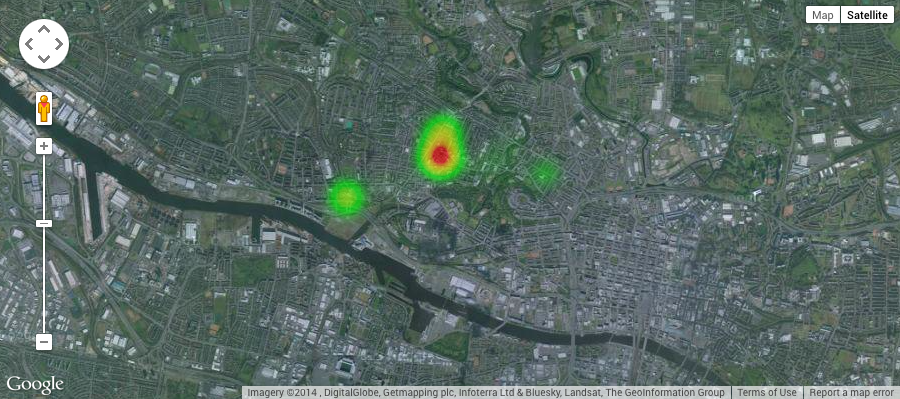
\includegraphics[scale=0.5]{images/screenshots/heatmapscreen.png}
\caption{\textbf{Screenshot showing a Heatmap of the City of Glasgow with data from usage of the Hotsteps pedometer application.}}
\label{impl:heatmapscreen}
\end{figure}

Heatmaps are maps that have many coordinates placed on them to determine levels of activity visually. Each Heatmap is created by adding all of the coordinates from the query period onto an embeddable Google Map frame defined using Javascript in the website code. The coordinates are added as an array of points and entered into the Map frame. The areas with the most data points appear as a deep red, areas with less data points as yellow/amber, and the areas with the least data points as a green colour. The less points featured on a specific areas the lighter the colour is. An example of a Heatmap is displayed in Figure \ref{impl:heatmapscreen}. 

To provide the Heatmaps, I used Google Maps' freely  available and usable library. This embeds a number of points on the map that are colour coded  It fits all of the criteria outlined in the design section, with options to invert the colours for people who suffer from colour blindness. Instead of red amber and green, the data points appear as cooler light blues, dark blues and purples.

\subsection{Web Technologies}

The site implementation includes a number of web technologies. PHP is used server side to track user sessions and query the Database in order to be able to create the appropriate cookies for the sites user. The cookies store a number of details about the account that is currently logged in, such as their username and userID both to present to the user and also to be able to seamlessly query the database wilst they use the website to present them with their data.

Javascript is used as the client side language. A great deal of the website functionality is implemented using Javascript. When each page on the website loads, it calls a number of JQuery requests. These JQuery functions send a POST request that will assemble the data that function requires in JSON format. This is then parsed by the Javascript function and displayed by that page in the HTML code.

\subsection{Cookies and Session Handling}

Due to the rejection of using a Web Application Framework (WAF) it was necessary to develop code that would be able to handle a users login across multiple page views, something standard HTTP cannot do. This is achieved through the usage of Cookies set using PHP executed server side as the page loads. When the user logs in, the password given is SHA-256 hashed and the PHP backend performs a query to check that the Username and SHA-256 Hashed Password match that of a registered user. If it does not, they are returned to the Login page and presented with a message saying that their username or password was entered incorrectly. 

If the user did enter an appropriate Username and Password, the PHP backend then queries the Database for the userID corresponding to that user, which is then saved in a Cookie, a small file that resides on the server to keep information between differing HTTP requests the user makes. If the user loads a new page, and that page needs to know the userID, it simply calls and request the value of the Cookie stored on the server.

\subsection{Website Pages}

\subsubsection{Home Page}

The Home Page, defined in \texttt{index.html}, displays aggregated data about all of the users of the site for that day. At the top Jumbotron, the number of steps made that day, week, month and al time is displayed. The page content is seperated 

\subsubsection{User Data}

This page allows the user to view their own personal data yo.  At the top of the page in a Bootstrap jumbotron is displayed the amount of steps the user has made in that chosen day, 
\subsubsection{Leaderboards}

The three different leaderboards pages, enable the user to view Daily, Weekly and Monthly leaderboards of the users with the highest step count. The leaderboards feature is designed so as to promote competition amongst users of Hotsteps, both increasing the users enjoyment, and also increasing both the quantity and the quality of the data.

\subsubsection{Create Heatmap}

This function allows the user to pick a range between two dates and view a special heatmap composed of all of the coordinate data from between those date ranges. This feature has a great number of potential uses.

\section{Security}

There were many aspects of security thought of when developing the system. In order to be able to use the system, the user must create their own account. This is a necessity due to the storage of user data, but also because of the sensitive location data that is stored amongst users of the application. If it was possible for another user to see a users personal information or location easily, the system would not be secure.

All of the user passwords stored on the system use SHA-256 encyption. As should be obvious, the plain text passwords themselves are never stored. As soon as they are entered, they are ran though the SHA-256 hashing algorithm, and all future references to the password are in that form. SHA-256 encryption is one of the most secure hashing algorithms known, and requires intense processing power to crack for any vaguely uncommon passwords.

Some concerns with security were noted from users of the application. One user noticed that when the user logs into the webpage, that their password is sent via plain-text to the web page that subsequently hashes the given password and checks whether their password is valid for the given user. This is vulnerable to a theoretical man-in-the-middle attack where a user may be packet sniffing. Due to timescale limitations, it was not possible to fix this given the remaining time, but if development on Hotsteps were to continue, then this should be fixed immediately using the more secure HTTPS instead of standard HTTP. If more users were to discover this, it would undermine confidence in the application, put people off from using the app, lessening the data received.

\section{Version Control}

Throughout development of the project, the Git version control system was used to provide version control for my codebase. This local Git repository was linked to the popular online based repository, Github.  Using GitHub provided numerous benefits to the development process. Firstly, the codebase was backed up remotely and safe in case of a major data-loss. Additionally, Git provides features such as Branching, which enables creation of different branches to aid development. For example, the main branch stores the major revisions that are known to work or at least be stable. If development proceeded on a more challenging aspect of the implementation, then development can be switched onto an 'experimental' branch so as to not endanger the code already in the main branch. Once the work on the experimental branch is complete and tested, this can then be merged back into the master branch.

\section{Problems Faced During Development}

One of the inital problems faced early in development was getting the Server and the Phone to be able to communicate with each other. This was due to network issues. The laptop used for development could create a Wi-Fi hotspot that the phone could access but Android did not recognise such a connection. After some trouble shooting it was discovered that tethering the mobile connection of the phone on the laptop would enable me to access the files located on the Apache server of the computer from the mobile phone using the computers IP address. This enabled development of the Application to be progressed on a local machine until the server was ready to host the files. 

When beginning to develop the application, problems were encountered in trying to understand and instantiate an object of type \texttt{StepCounter} to track the number of steps the user is making. The code as initally received included code to hook into a local database which I would not be using for the purposes of this application, and did not come with clear instructions in regards to implement it. After some trial and error and e-mails to the original author, it was discovered how to instatiate the class by setting a type Boolean \texttt{isSensoring} to be true whilst setting the Pedometer running.

%==============================================================================

\chapter{Testing}

\section{Hotsteps Testing}

One of the challenging aspects of this project was actually testing the application. Pedometers are hard to test in that you need to walk around for large periods of time in a realistic walking environment.

\subsection{Pedometer Testing}

\subsubsection{Step Counting Testing}

The testing of the actual Pedometer of the application is very important, since it was integral for the app to be counting the correct amount of steps. The testing process used a commercial equivalent on the Android platform in order to compare my results. The commercial application that used was Pedometer, as of March 2014 the highest rated Pedometer application on the Google Play Store. Testing involved walking around as usual with both pedometers running. Given that Pedometer is a commercial application, we can make reasonable assumptions about its accuracy but it was also compared with another equivaelent application to be sure of its efffectiveness also.

The results were fairly good with a margin of error. Whilst it is a little out, this is not important in the grand scheme of things.

\subsubsection{Battery Life Testing}

In order to test users battery life whilst using the application, I asked users who had had the application for a longer time than the other evaluators their feelings on the battery life used by the application. Most felt fairly satisfied with the battery life, with no one noticing any particular worsening of phone battery life, though in some cases where users had been playing about with the leaderboards and statistics, and continually refreshing, then one user reported it had taken about 20 percent of the battery life in that charge cycle, though on average it seems to settle about 6 percent of battery use when running in the background.

\subsubsection{Found Bugs}

An unsolved bug was uncovered that meant on occasion the application would not function correctly and would crash upon login. This was revealed to be a problem with Location Services, and it has not been uncovered whether it is a bug on the applications code or the API. On all occasions so far, the bug is fixed by having the user turn of and on location functionality on their device and restarting their device. Before a larger scale evaluation was carried out, it would be critical to reveal the cause of and fix this bug as it is fairly severe when it does occur and negaatively impacts people's view of the application.

\subsection{Backend Testing}

It was necessary to test the back end of the application. This was mostly tested though the website and application, and see if the results from querying the database were generally correct. The testing was mostly correct.

\subsection{Website Testing}

In order to test the website, the website was used with a number of different accounts and tested to see if all of the JQuery queries achieved the correct result for that user. A number of bugs were uncovered using this method.

%==============================================================================

\chapter{Evaluation}

\section{User Evaluation}

In order to reach conclusions about the effectiveness of the project, what users liked and disliked about the application it was necessary to carry out a user evaluation. Ideally, given a longer project duration this evaluation would have consisted of a small scale evaluation to get micro-feedback and a larger scale evaluation. The proposed larger scale evaluation would have involved releasing the application on the Google Play Store or similar method of mass software release. Larger data sets would have been achieved and it could have tested how large scale the application could handle.

Given the limited timescales involved, this larger scale evaluation was considered unfeasible, and therefore only the smaller scale evaluation went ahead. In future, a larger scale evaluation would need to take place to harvest data and opinions from a much larger and more representative group of people.

The goals of the evaluation revolved around three aspects. Given that the goal of Hotsteps is to promote an environment where users are motivated to use the application in order to provide the data, there were three aspects that the system has to be successful at to promote future use. These are:

\begin{enumerate}

\item{Is the app interesting enough? If the app is not interesting enough and does not have enough/has the wrong features, then users will not want to use the app in the future. Carrying out the evaluation should establish whether users think the app is interesting enough, and what features could be added to make it more interesting}

\item{Does using the application greatly negatively impact battery life? If the user feels that the app is greatly negatively impacting their battery life, leaving them unable to do what they would like to do with their phone? If this is a very negative impact, users will simply delete the app and therefore limiting the amount of data received.}

\item{Privacy concerns - the app tracks user locations whilst using the app, as well as the number of steps the user takes every 15 minutes. Some users may feel uncomfortable with this, and therefore will not use the app, whilst some users will be OK with this, and as such this would not put them off using the app. The evaluation should discover the range of feelings about this, and hopefully discover strategies that could be used in future versions of the application to mitigate any concerns that may occur.}

\end{enumerate}

\section{Evaluation Strategy}

Upon completion of development of the app and website, it was necessary to carry out a user evaluation to determine from the eyes of end users how well I had achieved what I set out to do and what could be implemented in future from the eyes of the users of the application.

When thinking about participants to use in the evaluation, it was necessary to consider a wide range of users so that the evaluation reflected opinions from a number of different groups of people. There were a number of instant limitations to the group of users that could take part in the user evaluation. The application developed only works on Android devices with Android version 3.0 and above. The limitation was chosen based upon updated UI guidelines and technology introduced with that update. Therefore, the evaluation sample users were fifteen people - five women and ten men, with a variety of age groups ranging from 18 to 53. One concern is the somewhat lower prevalence of women in the sample - future evaluation might wish to have slightly more women than men in order to balance out the results. 

One issue with the evaluation as carried out was that the participants were not being compensated for taking part in the user evaluation, and a worry was that the users would not bother to use the application for any length of time. This could also be seen as a good thing, for, if example, the users did not feel they had to sugar-coat their feelings because they were being recompensated.
 
Due to the theoretical privacy concerns raised by the application, it was necessary to gather user consent from all of my participants. This was carried out in a two stage process - 1) When the user had agreed to be a part of the evaluation, they were made to read and sign a form that explained to them that the application and website would be tracking information about the number of steps they made, and location data about where they used it. It was also explained to them the reasons for carrying out the evaluation, my name and contact address for if they wanted to contact me about any concerns or questions that they had. Finally, it was explained to them that they could leave the evaluation at anytime if they felt uncomfortable, and that there should be no embarrassment for doing so.

During the user testing stage, there was regular bug updates and features added to the application in response to user feedback.

The pedometer application developed was then evaluated. The main thrust of the evaluation was based upon the website, given that the application was designed to work in the background, going about its business.

The conclusion was then written. I concluded stuff. That stuff was good.

\section{Evaluation Execution}

The website evaluations took place in a controlled lab environment, on a lab PC running Scientific Linux and the latest version of the open-source Chromium web browser. Participants were asked to download the latest version of the application APK onto their device a day or so before the lab based experiment, and were asked to use the app for a day or so during their day to day business. This fulfilled two functions. It allowed the user to have experience of using the application and help them form their opinions of the app. Additonally, it allowed the user to harvest data before the evaluation began giving the enough data in their account to be able to use all of the features of the website as intended.

When the evaluation began users were asked to fill out a form thanking them for taking part in the evaluation and explaining to the user what would be happening in the evaluation, that think-aloud would be in operation and they could speak their thoughts as they operated the website. They were then given a sheet that included a list of operations that the user might want to try out. This means that the user had an idea of what they could use the website to do but that the evaluation was not as rigid as a standard walkthrough. This gives the user a greater idea of how it would feel in real usage. The user was given as long as they felt that they needed to use the website. This was usually around 5 minutes long for most of the users.

Once the user had completed the website evaluation, they were asked to fill out the questionnaire and then carry out a short interview that lasted about 5 minutes. This interview was recorded for the purpose of being able to use and build upon the exact information glaned later. The aim of having both the questionnaire and the verbal interview was to have both qualitative and quantitative data. Qualitative data is data involving numbers. Qualitative data is more rich, text based with opinions, likes and dislikes included. By combining both pieces of data, it was possible to get a good viewpoint of how users feel about the app, their likes, dislikes and what can be improved.

Once the evaluation was over the user was thanked for taking part in the evaluation, and asked to email about any questions or concerns they may have had. Once the final report was completed, they were informed that they would have access to the report and read the conclusions if they so desired.

\section{Evaluation Questions}

The questions asked of the users during the evaluation were as follows:

1: Do you enjoy using Hotsteps at its current stage of development?

2: Hotsteps would motivate me to walk more in the future.

3:  Would you like to continue using Hotsteps from now on?

4: Did you feel that the Android application was easy to use?

5: Did you feel that the Android application needed additional features?

6: Did you feel that the website was easy to use?

7: Did you feel that the Website needed additional features?

8: How concerned are you about privacy issues whilst using Hotsteps?

Any other thoughts about Hotsteps? What new features would you like, likes/dislikes, privacy concerns?

\section{Evaluation Results}

N.B The numerical results from the evaluation are given in Appendix A.

The results of the evaluation suggest that Hotsteps has some merit in doing what it sets out to do, but that it would require lots of additional work to live up to users full expectation. Additionally, some users had a number of privacy concerns about Hotsteps tracking their locations, though users helped establish a number of ways that this could be alleviated.

The results were overall a mixed bags. Users liked the ideas behind the application, but were less optimistic about some of the implementation aspects. For example, users were generally impressed with the large scale nature of the application and liked the usage of the website to view the Heatmaps, but some users also noted a lack of features and some bugs during the evaluation that limited their enjoyment.

Users generally expressed a high degree of concern over the location tracking functionality of the application whilst still liking the feature. The main ethics concern from evaluated users was not necesssarily their movements being tracked on a Heatmap in general, but that in certain circumstances where little usage had occurred it was possible to enter large amounts of data in a specific point such as 

Given the lack of larger scale evaluation, some of the conclusions made in this report would require further investigation on more users before being made final. More data would need to be uncovered about the likelihood of increasing walking activity and usage of the app, but the evaluation carried out could inform the areas of focus in the larger scale evaluation. 

%==============================================================================

\chapter{Conclusion}

In conlusion, the project was fairly successful.

I developed an app and evaluated it. The evaluation went well.

I developed a website and evaluated it. The evaluation went well.

I developed a back-end and tested it.

Then I wrote this dissertation.

Then I was finished, thank fuck. The app is pretty decent, but it has a lot of work before it could be considered final, many more features need to be added and the android app given a polish.

The application made shows a degree of promise, but will require additional development time and a larger scale evaluation before any final conclusions can be made. In the mean time, there are a number of features that can be added based upon user feedback, and also tackle some of the privacy issues that arised during the user evaluation. Users generally liked and enjoyed the service, and were impressed by the Heatmap functionality on the website, but a number noticed some simple design issues and bugs that affected their enjoyment of the system.

Another issue that could be used 

\section{Future Work}

In future, there are a number of features that I feel should be implemented, as backed up by my user study. Whilst the application is programmed to be large scale, if the large scale became properly large then the current set up might have a very hard time. In order to test this, there are numerous assumptions made about the app that have not been properly tested.

Given that a large percentage of smartphone users use the iOS mobile Operating System, there are a large number of prospective users who are simply unable to use the application whilst there is no iOS version of the application. If the app became popular or it was decided that more users were needed, an iOS version could help facilitate this. One thing that it would be necessary to guarantee is that the level of functionality could be guaranteed across any of the platforms that the app runs across - users must be able to have the same accounts between all of the different platforms, and be able to log into the website and see the shared data regardless of what platform it originated on.

Once this was implemented, it would be good at looking at extending the functionality of the apps themselves - the evaluation suggested that users think that these are fairly bare-bones and lacking in features. The first step in executing this would be to move the functionality of the website to also be available on the applications. Having access to richer data with the website would make the application much more useful than it is currently and stuff.

Further work may also be needed to improve the look and feel of the Heatmaps that are shown in the website. Currently, these appear as clusters of 'blobs' in the map, not as a contiguous line that would be preferred given the data provided to the map. It may be possible to fix this using the current Google provided library, or it may be necessary to look into other libraries available or possibly development of a custom solution to closely adhere to the necessary functions required by the system.

Additionally, the users concerns over privacy would need to be addressed. There are a number of ways that this could be achieved.

*LIST ALL OF THE FEATURES HERE*

%==============================================================================

\chapter{Appendix}

\section{Bibliography}

Luis von Ahn and Laura Dabbish. 2004. Labeling images with a computer game. In Proceedings of the SIGCHI Conference on Human Factors in Computing Systems (CHI '04). ACM, New York, NY, USA, 319-326.

Marek Bell, Stuart Reeves, Barry Brown, Scott Sherwood, Donny MacMillan, John Ferguson, and Matthew Chalmers. 2009. EyeSpy: supporting navigation through play. In Proceedings of the SIGCHI Conference on Human Factors in Computing Systems (CHI '09). ACM, New York, NY, USA, 123-132.

Swan, Melanie. "Emerging patient-driven health care models: an examination of health social networks, consumer personalized medicine and quantified self-tracking." International journal of environmental research and public health 6.2 (2009): 492-525.

Li, Ian, Anind Dey, and Jodi Forlizzi. "A stage-based model of personal informatics systems." Proceedings of the SIGCHI Conference on Human Factors in Computing Systems. ACM, 2010.

HERMAWATI, S. and LAWSON, G., 2013. Managing obesity through mobile phone applications: a state of the art review from a user-centred design perspective Personal and Ubiquitous Computing. 2014

A Morrison, O Brown, D McMillan, M Chalmers.Informed Consent and Users' Attitudes to Logging in Large Scale Trials. CHI Extended Abstracts, 1501-1506, 2011.

Krumm, J. A survey of computational location privacy, Personal Ubiquitous Computing, 13(6) 391-399 (2009)


\section{Evaluation Results - Quantitative Data}

\begin{figure}[H]
\centering
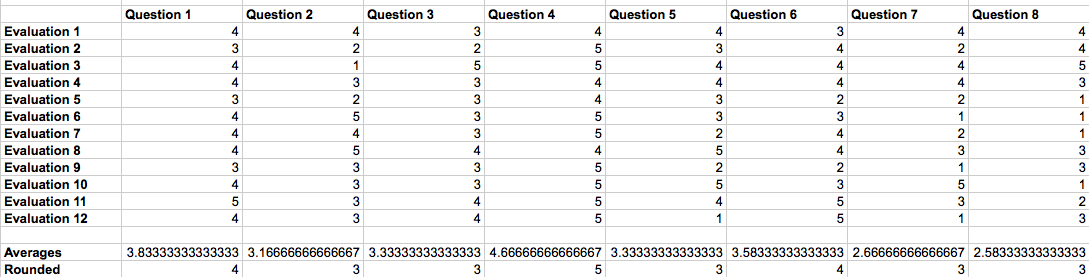
\includegraphics[scale=0.4]{images/screenshots/resultsscreen.png}
\caption{\textbf{Overview of the results of the evaluation and the questions given in Section 7.0.7}}
\label{apndx:resultsscreen}
\end{figure}
 
\section{Glossary of common terms and abbreviations used}

Android - An open-source Mobile Operating System with development lead by Google. Currently the most popular Mobile OS, with XX percent of the market as of March 2014. The basis of Android is the Android Open-Source Project, which consists of the Operating System and a limited number of Open-Source applications. On top of AOSP is Google Play services, which provides a number of Google based applications and access to the Google Play Services API.

Google Play Services - An API that enables Android developers to access Google provided services such as Mapping. In the Android application there are regular calls to this API to request the current location.

Tethys - the server located within the school that currently hosts the PHP backend and Database of Hotsteps.

Javascript - Client side language to provide web functionality.

PHP - (A recursive backronym for PHP: Hypertext Preprocessor) is a Server side scripting language, but it can also be used as a general purpose programming language. Handles database querying, cookies and session handling. One of the most common server side languages, installed on the vast majority of the world'sa web servers.

mySQL - An open-source relational Database Management System (DBMS). Very common usage.

HTTP - Hyper Text Transfer Protocol (HTTP) enables clients and servers to talk to each other using structured text to relay information.

POST Request - Information sent via HTTP while requesting a website. More secure than GET requests as the information is not visible as in GET requests.

GET Request - Information sent via HTTP to a server. The information sent is encoded in the URL, meaning it is less ecure than POST requests.

Apache Server - Software to provide server functionality. The server used to provide the website, Database and PHP scripts for the project are hosted on an Apache server.

APACHE License - An open-source licence by the Apache foundation. Software used in this project, such as Android and Apache web server, is released under this license.

Accelerometer - Detects acceleration. Built into every modern smartphone and is used in the Application as part of the step detection.

Gyroscope - Detects movement in space, this is also used to detect the users steps in the Pedometer.

APK - The filetype for Android application files. Consists of the application and a special manifest file. Similar to Java jar files.

LIST STUFF HERE!!!!

\end{document}